\section{Experiments}
\label{sec:exp}

\subsection{Experimental Setting}
\label{sec:setting}

\noindent\textbf{Benchmark.}\quad We conduct experiments on BEAT~\citep{liu2022beat}, which pairs natural speech with ARKit coefficients captured at 60\,Hz and is therefore directly usable for an Audio2ARKit comparison. We use its English subset and screen it by rendering the captured coefficients against the audio, discarding sequences with tracking failures or audible misalignment, since a reference that does not match its own audio cannot support training or evaluation. The retained data are split by speaker into 176 training, 40 validation, and 61 test sequences, and semantic segmentation yields 15{,}655 training, 2{,}858 validation, and 3{,}000 test units. Appendix~\ref{app:dataset} details the procedure.

\noindent\textbf{Metrics.}\quad We report five metrics covering accuracy, distribution, and appearance, where MSE and MAE measure frame-level coefficient error. Fr\'echet distance (FD) measures the discrepancy between predicted and reference motion distributions in a feature space, and Wasserstein inception distance (WInD) follows the protocol of SAiD~\citep{park2023said}. Lip landmark distance (LMD) measures the mean Euclidean distance between 2D mouth landmarks in paired rendered videos, and is the only metric outside the coefficient domain, which makes it independent of the geometric term inside our reward.

\noindent\textbf{Baselines.}\quad We compare AudioMouth with four Audio2ARKit methods, namely LAM-A2E~\citep{lam}, NVIDIA Audio2Face-3D~\citep{chung2025audio2face}, SAiD~\citep{park2023said}, and SentiAvatar~\citep{jin2026sentiavatar}, covering real-time production pipelines, diffusion-based generation, and sentence-level planning. SAiD is fine-tuned from its public checkpoint on our training split, while the other three are evaluated with released weights because their training code or data is unavailable. Two asymmetries follow. The three unadapted baselines never see our speakers, and all four consume audio alone while AudioMouth also consumes the transcript and phonemes its formulation requires. Table~\ref{tab:main} therefore compares formulations as they are distributed, and the Audio Only ablation of Sec.\ref{sec:ana_conditioning} is the matched-input reference under our own backbone and data.

\noindent\textbf{Configuration.}\quad We build AudioMouth on Qwen3-Omni-30B-A3B-Instruct~\citep{xu2025qwen3omni} and adapt it with LoRA~\citep{hu2021lora} on the language decoder, keeping the audio encoder and multimodal alignment modules frozen so adaptation concerns only how motion is generated. Preprocessing combines automatic speech recognition with SAT~\citep{frohmann2024segment}. Supervised fine-tuning and GRPO each run for four epochs, refinement samples six candidates per prompt, all training and inference use NVIDIA A100 GPUs, and predictions are rendered with MetaHuman~\citep{metahuman}. Appendix~\ref{app:training} reports the full configuration.

\subsection{Main Results}
\label{sec:main_results}

\begin{table}[t]
\centering
\caption{AudioMouth improves every metric over four Audio2ARKit methods on the subject-disjoint BEAT test split, with the largest margins on the distributional metrics FD and WInD. All metrics are lower-is-better. FD, WInD, and LMD are mean $\pm$ sample standard deviation across evaluation scripts, \textbf{bold} marks the best result per column, and \textcolor{blue}{$_{-x\%}$} is the relative reduction over the strongest baseline in that column.}
\label{tab:main}
\vspace{-1mm}
\scriptsize
{\renewcommand{\arraystretch}{1.12}
\begin{tabular*}{\textwidth}{@{\extracolsep{\fill}} lccccc @{}}
\toprule
\textbf{Methods} & \textbf{MSE $\downarrow$} & \textbf{MAE $\downarrow$} & \textbf{FD $\downarrow$} & \textbf{WInD $\downarrow$} & \textbf{LMD $\downarrow$} \\
\midrule
LAM-A2E                       & $0.023$ & $0.109$ & $38.403 \pm 10.149$ & $41.751 \pm 10.885$ & $7.648 \pm 0.497$ \\
Audio2Face-3D                 & $0.020$ & $0.106$ & $25.228 \pm 3.560$  & $29.879 \pm 4.454$  & $7.879 \pm 0.438$ \\
SAiD                          & $0.021$ & $0.108$ & $58.357 \pm 21.580$ & $62.256 \pm 21.911$ & $7.651 \pm 0.504$ \\
SentiAvatar                   & $0.022$ & $0.106$ & $40.609 \pm 10.277$ & $42.153 \pm 10.542$ & $8.131 \pm 1.005$ \\
\midrule
\rowcolor{gray!15}
\textbf{AudioMouth} & $\mathbf{0.006}$\,\textcolor{blue}{$_{-70\%}$} & $\mathbf{0.053}$\,\textcolor{blue}{$_{-50\%}$} & $\mathbf{10.820 \pm 2.635}$\,\textcolor{blue}{$_{-57\%}$} & $\mathbf{16.513 \pm 3.584}$\,\textcolor{blue}{$_{-45\%}$} & $\mathbf{6.249 \pm 0.723}$\,\textcolor{blue}{$_{-18\%}$} \\
\bottomrule
\end{tabular*}
}
\vspace{-4mm}
\end{table}

\noindent\textbf{Capability on Speech-Driven Coefficient Prediction.}\quad
We first evaluate AudioMouth on the BEAT test split to assess its \emph{coefficient-level articulation accuracy}, where every method receives the same speech and predicts the same 32 channels over the same speaking intervals. We compare it with the four Audio2ARKit baselines of Sec.\ref{sec:setting}. As shown in Table~\ref{tab:main}, AudioMouth achieves state-of-the-art performance among Audio2ARKit methods on all five metrics, substantially reducing MSE by 70\% and Fr\'echet distance by 57\% relative to the strongest baseline in each column. More importantly, the gains are not uniform across metric types. Frame-level MSE and MAE separate the four baselines by at most 15\%, which indicates that predicting the dominant near-zero coefficients is easy for any reasonable regressor and that frame-level error alone cannot distinguish these methods. The distributional FD and WInD spread the same baselines over a factor of two, showing that what differs between them is whether the predicted motion occupies the same region of motion space as real speech. In contrast, AudioMouth improves most on exactly these distributional metrics, which stems from articulation grounding, since naming the control a phoneme drives constrains which channels move and not only how much error each channel accumulates. Its FD standard deviation is also the smallest of all methods, so the advantage holds across scripts. Overall, AudioMouth's strong results on BEAT highlight its advanced capability in producing mouth motion whose channel activation pattern matches real articulation.

\begin{figure*}[t]
    \centering
    \vspace{-2mm}
    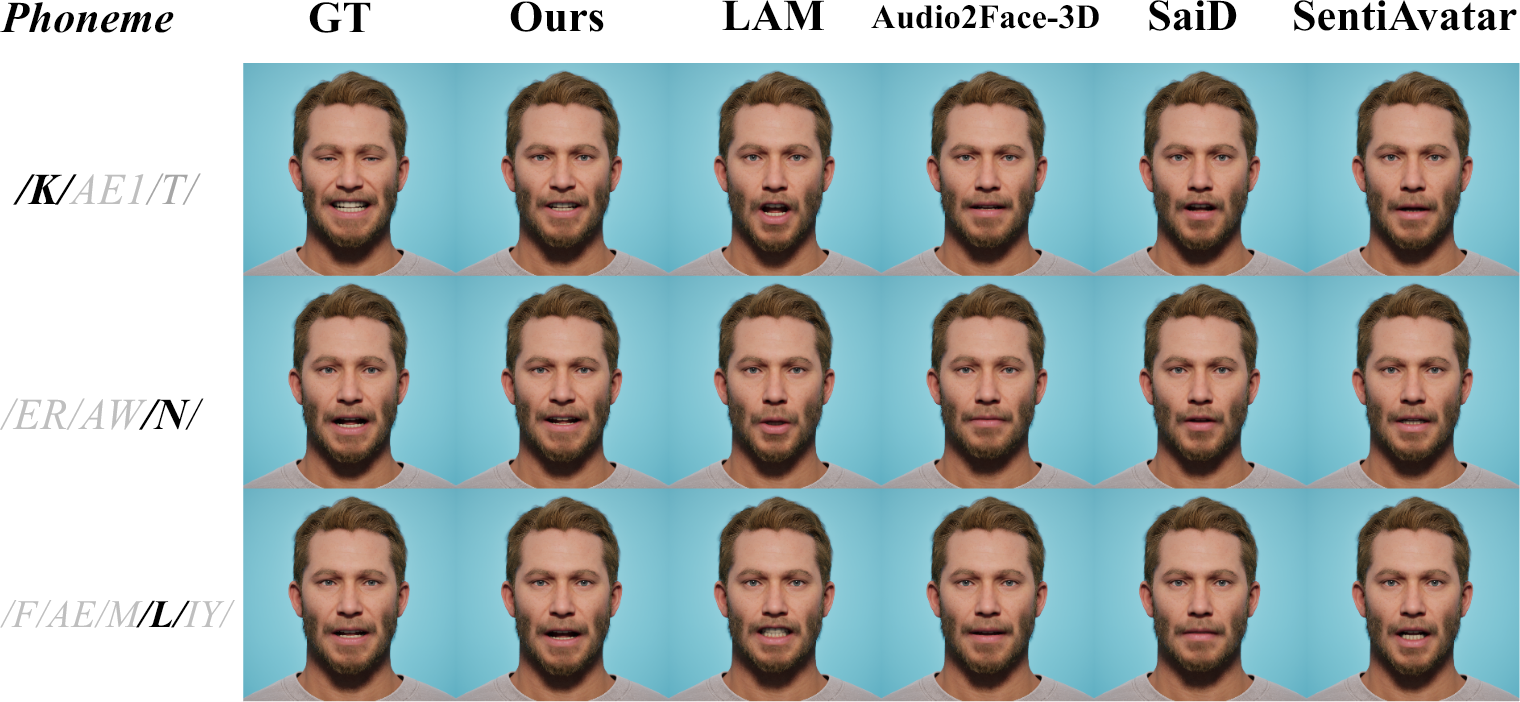
\includegraphics[width=0.9\linewidth]{comparison.png}
    \vspace{-2mm}
    \caption{AudioMouth reproduces the articulatory target of each phoneme, closing the lips on the bilabial in ``family'' and opening the jaw on the open vowel in ``cat'', where baselines keep a partially open, weakly differentiated mouth shape. The leftmost column shows the phoneme context with the active phoneme in bold.}
    \label{fig:comparison}
    \vspace{-3mm}
\end{figure*}

\noindent\textbf{Capability on Rendered Mouth Appearance.}\quad
Coefficient accuracy is only useful if it survives rendering, so we render every prediction with MetaHuman and measure LMD against the rendered reference, the one metric computed outside the coefficient domain. As shown in Table~\ref{tab:main}, AudioMouth reduces LMD by 18\% relative to the best baseline, a smaller margin than the 57\% it achieves on FD. This narrower margin stems from how the two metrics are formed, because LMD averages a landmark distance over all frames and is dominated by the many frames in which the mouth is nearly closed for every method, while FD is sensitive to the shape of the whole motion distribution. Figure~\ref{fig:comparison} shows where the remaining difference is visible. On the bilabial in ``family'' the baselines leave a gap between the lips, and on the open vowel in ``cat'' they produce a moderate opening for a sound requiring a wide one, whereas AudioMouth reaches the articulatory target in both cases. In contrast, AudioMouth is told that bilabials close the lips, so it reproduces a named articulatory event instead of a numerical average over acoustically similar sounds. Overall, AudioMouth's strong results under rendering highlight its advanced capability in carrying coefficient-level accuracy through to the visible face, with the clearest gains on the phonemes whose articulation is most constrained.
